\chapter{Da dove vengono i numeri complessi}

I numeri complessi vengono dalla ricerca delle soluzione di una equazione cubica da parte di Cardano, cioè le soluzioni di un equazione del tipo:
$$x^3+ax^2+bx+c=0$$
Applicando il cambio di variabile $x=x'-\frac{a}{3}$ otteniamo un equazione sempre di terzo grado, ma nella quale non compare più il termine di secondo grado. A tale equazione applichiamo nuovamente un cambio di variabili $x'=kx''$;ci riconduciamo quindi ad un equazione del tipo:
$$x^3+-3x+a=0$$
A questo punto possiamo scrivere il polinomio come il prodotto di tre binomi di primo grado $(x-x_1) (x-x_2) (x-x_3)$ dove $x_1, x_2$ e $x_3$ sono le tre soluzioni cercate.
Esse devono soddisfare le condizioni:
\begin{itemize}
\item $x_1+x_2+x_3=0$, infatti manca il termine di secondo grado.
\item $-x_1 x_2 x_3=a$, cioè il termine noto.
\end{itemize}
In contemporanea all'uscita della soluzione di Cardano, Ferrari pubblica la sua soluzione per un equazione di quarto grado, procedendo in maniera simile a Cardano: partendo dall'equazione $x^4+ax^3+bx^2+cx+d=0$ ed effettuando la sostituzione $x=x'+\frac{a}{4}$, si ottiene un'altra equazione nella quale non compare il termine di terzo grado.

\section{Il campo complesso}

L'assiomatizzazione del campo complesso, introdotto per la prima volta da Eulero e successivamente rappresentato graficamente come punti sul piano da Gauss, è dovuta ad Hamilton.
Possiamo vedere un numero z complesso come un punto nel piano $\R \times \R$, quindi con coordinate $(x;y)$. Questo tipo di rappresentazione fa sì che i numeri complessi godano di tutte le proprietà della somma, definita come:
$$z+z'=(x;y)+(x';y')=(x+x';y+y')$$
Infatti per questa scrittura valgono le proprietà associativa, commutativa, esiste l'elemento neutro -rappresentato dal vettore nullo $(0;0)$- ed esiste l'elemento opposto -rappresentato da $(-x;-y)$-.
\\
E' facile osservare che la somma di cui si sta trattando in questo caso è una somma vettoriale; infatti, rappresentando i numeri complessi con dei vettori che uniscono l'origine con il punto di coordinate $(x;y)$, si utilizza la regola dei parallelogrammi.
\\
\\
\\
\begin{figure}[h!]
  \centering
    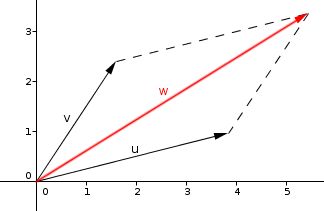
\includegraphics[width=0.5\textwidth]{immagini/sommavettori.png}
\end{figure}

Invece il prodotto fra due numeri complessi viene definito come il prodotto vettoriale, cioè:
$$zz'=(x;y)(x';y')=(xx-yy'';x'y+xy')$$
Anche in questo caso valgono tutte le proprietà del prodotto: commutatività, associatività, esistenza dell'elemento neutro $(1;0)$ e, se $z$ è non nullo, esiste l'inverso $\frac {1}{z}$ .
\\
Oltretutto, vale la proprietà distrubutiva fra il prodotto e l'addizione, cioè:
$$(z_1 +z_2 )z_3 =z_1 z_3 + z_2 z_3$$
La seguente proposizione è stata dimostrata da Hamkel:
\begin{teorema}
$\C$  è il più generale campo che soddisfa tutte le proprietà algebriche, cioè non posso costruire un campo più grande che mantenga verificate tali proprietà.
\end{teorema}
Questo vuol dire che ogni passo avanti corrisponde alla perdita di validità di una proprietà algebrica (ad esempio, nei quaternioni\footnote{Corpo non commutativo che, similmente al campo complesso, ha delle unità ''immaginarie'' (come $i$ per i complessi). Si veda \url{https://it.wikipedia.org/wiki/Quaternione} per approfondimenti (tranquilli, non fa parte del corso).} non vale la commutatività).
\\
Gli elementi del tipo $(x;0)$, cioè gli elementi del campo reale, formano un sottocampo del campo complesso, cioè $\R$ è un sottocampo di $\C$. Questo porta a definire il prodotto per uno scalare:
$$x(x';y')=(x;0) (x';y')=(xx';xy')$$
Sfruttando questa proprietà, vediamo che possiamo scrivere un qualsiasi numero complesso come:
$$(x;y)=x(1;0)+y(0;1)=x+iy$$
Dove $i$ rappresenta l'unità dell'asse immaginario, cioè il vettore (0;1). Si noti che $i$ è anche la radice di -1; infatti:
$$i^2=(0;1) (0;1)=(0-1;0+0)=(-1;0)=-1$$

Definiamo ora il numero complesso coniugato, cioè quel numero (complesso) tale che, se $z$ è scritto come $x+iy$, si ha che il complesso coniugato risulta:
$$\overline{z}=x-iy$$
Risulta ovvio che $\overline{\overline{z}}=z$.

Infine, definiamo il modulo di un numero complesso $z$ come la somma in quadratura della parte reale e della parte immaginaria, cioè:
$$|z|=\sqrt{x^2+y^2}\geq0 \, \, \, \forall z$$
\clearpage
Vediamo ora alcune proprietà dei complessi:
\begin{itemize}
\item $\overline{z_1 z_2}=\overline{z_1} \, \overline{z_2}$
\item $Re(z)=x=\frac{z+\overline{z}}{2}$
\item $Im(z)=y=\frac{z-\overline{z}}{2i}$
\item $|z|=0 \iff z=0$
\item $|z_1 z_2|=|z_1| |z_2|$
\item $|z_1 + z_2| \leq |z_1| + |z_2|$
\end{itemize}
%%Regola del parallelogramma%%
Introduciamo ora due nuovi tipi di rappresentazione del numero complesso $z$. La prima tipologia è detta rappresentazione polare; si ha che:
$$z=x+iy=|z| \left(\frac{x}{|z|}+i \frac{y}{|z|} \right) =|z|(cos(\theta) +i sen(\theta))$$
Infatti sia la parte reale sia la parte immaginaria sono (in modulo) $\leq 1$, e la somma dei loro quadrati dà 1; quindi,  essi rappresentano il seno e il coseno di un angolo $\theta$ tale che $tg(\theta)=\frac{y}{x}$ .
\\
\\
Il secondo tipo di rappresentazione è chiamata rappresentazione esponenziale ed è strettamente legato alla rappresentazione polare; infatti possiamo scrivere:
$$z=|z| (cos(\theta) +i sen(\theta))=|z| e^{i \theta}$$
Questa modalità di rappresentazione dei complessi ci è molto utile nel prodotto fra due numeri complessi; infatti, scrivendo $z_1$ e $z_2$ in forma esponenziale, risulta facile verificare che $z_1 z_2=|z_1||z_2|(cos(\theta + \phi) +i sen(\theta + \phi))$, dove $\theta$ e $\phi$ sono gli angoli relativi ai due numeri complessi presi in considerazione.

Insieme alla rappresentazione esponenziale, introduciamo la funzione argomento principale $Arg(z)$ che associa ad un numero complesso un angolo $\theta \in (-\pi;\pi]$; possiamo quindi scrivere il numero complesso $z$ come:
$$z=|z| e^{i \, Arg(z)}$$

Il motivo per cui $-\pi$ non è incluso nell'intervallo di definizione della funzione argomento principale è legato al fatto che , se così non fosse, avremmo un indecisione sulla scelta del valore dell'angolo da associare; infatti, utilizzando dei semplici limiti, si nota che sul semiasse negativo delle ascisse la funzione $Arg(z)$ presenta una discontinuità di $2i\pi$.
\\
\\
Una formula molto importante per muoversi nel campo complesso è la \textbf{formula di De Moivre}:
$$(cos\theta + i sen\theta)^n =cos(n\theta) + i sen(n\theta)$$
Essa risulta ovvia una volta che si è riscritto il numero complesso in forma esponenziale.\\Vediamo ora come si comporta la funzione esponenziale nel campo complesso; abbiamo che:
$$e^z=e^{x+iy}=e^x e^{iy} =e^x (cos(y)+isen(y))$$
Le proprietà dell'esponenziale nel campo complesso sono:

\begin{itemize}
\item $\overline{e^z}=\overline{e^x e^{iy}}=\overline{e^x} \, \overline{e^{iy}} =e^x e^{-iy} =e^ {\overline{z}}$
\item $e^z =0$ non ha soluzione
\item $e^{z+2i\pi}=e^z$ cioè l'esponenziale è una funzione periodica sull'asse immaginario
\end{itemize}

La funzione esponenziale, infine, è molto utile per riscrivere le funzioni trigonometriche nel campo complesso:

\begin{itemize}
\item $cos(z)=\frac{e^{iz}+e^{-iz}}{2}$
\item $sen(z)=\frac{e^{iz}-e^{-iz}}{2i}$
\item $cosh(z)=\frac{e^z+e^{-z}}{2}$
\item $senh(z)=\frac{e^z-e^{-z}}{2}$
\end{itemize}

